%!TEX root = ../../../FYP_Dissertation.tex


%===============================================================================
% Methodical Accelerator Design
%===============================================================================

\subsection{Lua}
\label{Subsec:Lua}

\begin{wrapfigure}{R}{0.3\textwidth}
    \centering
	
\includegraphics[width=0.25\textwidth]{./Images/Lua.eps}
    % \caption{MAD-NG application}
    \label{fig:lua-logo}
\end{wrapfigure}

Authors claims that Lua is a powerful, efficient, lightweight, embeddable
scripting language. It supports procedural programming, object-oriented
programming, functional programming, data-driven programming, and data
description. Lua combines simple procedural syntax with powerful data description
constructs based on associative arrays and extensible semantics. Lua is
dynamically typed, runs by interpreting bytecode with a register-based virtual
machine, and has automatic memory management with incremental garbage collection.
It has been designed, implemented, and maintained by a team at \emph{PUC-Rio}
(See official website for more info \cite{lua}).


%
%===============================================================================
% Methodical Accelerator Design
%===============================================================================

\subsection{LuaJIT overview}
\label{Subsec:LuaJIT-overview}

\begin{figure}[H]
    \centering
	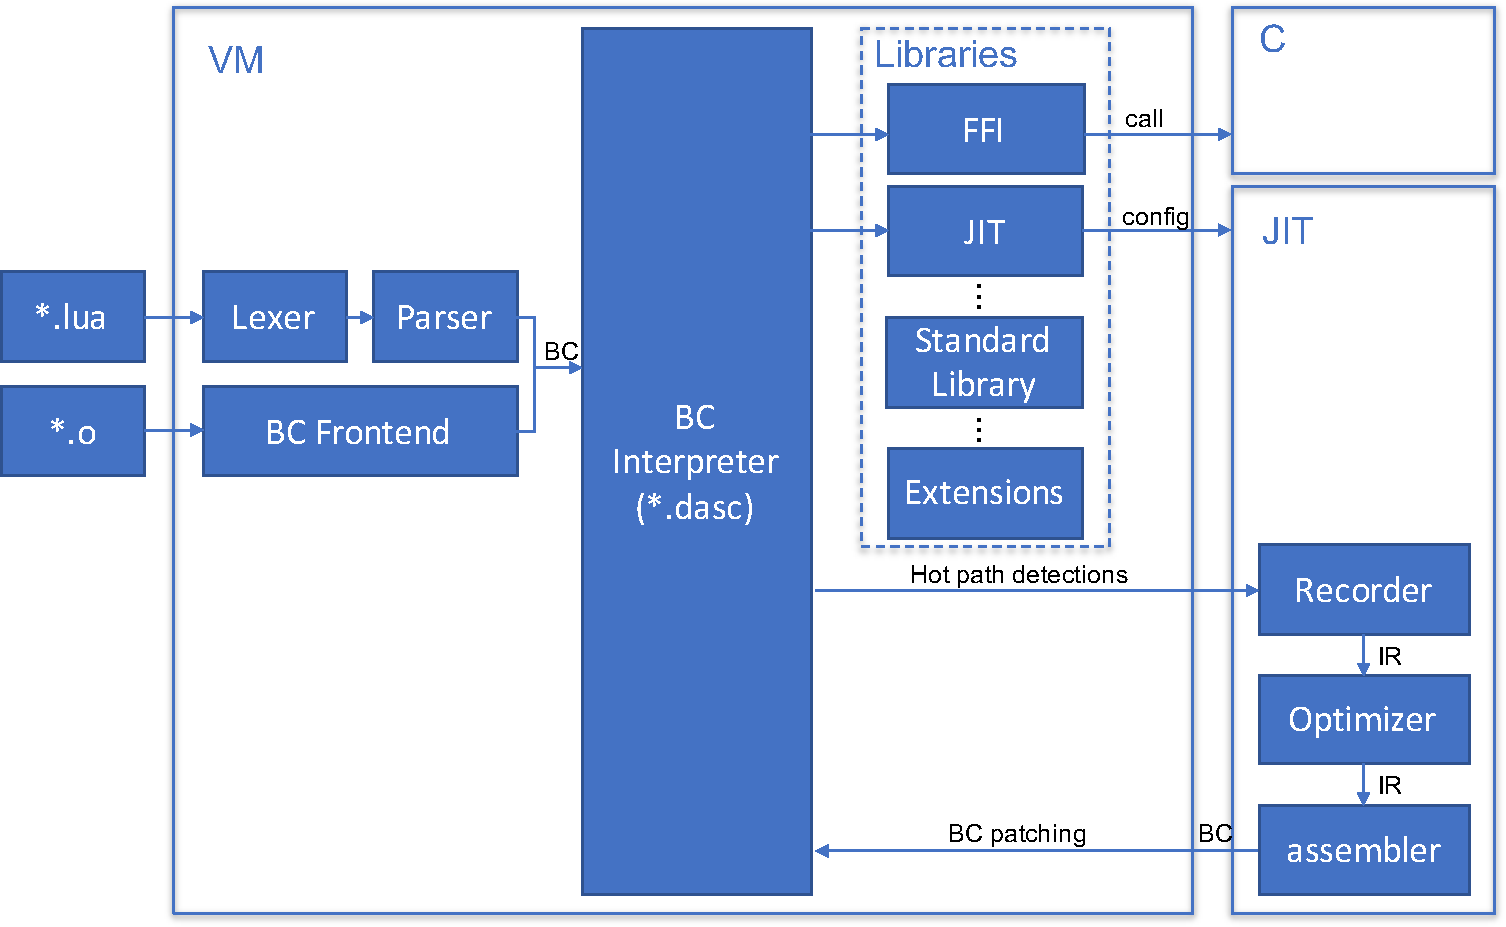
\includegraphics[width=\textwidth]{./Images/LuaJIT.pdf}
    \caption{Schematic view of LuaJIT internals}
    \label{fig:mad-graph}
\end{figure}
% - one paragraph per part with link to appropriate chapter
